\documentclass[usletter, 12pt]{article}
\usepackage{amsmath}
\usepackage{enumitem}
\usepackage{graphicx}
\graphicspath{ {images/} }


\begin{document}


\begin{enumerate}[leftmargin=0em, label=\textbf{\arabic*}.]
  \setcounter{enumi}{1} % remove this if you want to add other solutions 
  \item \textbf{Solution}:\\
    \begin{enumerate}[leftmargin=2em, label=(\textbf{\alph*})]
    \item Plot $\displaystyle{\frac{1}{[2+\cos(3\phi)]^2}}$ from $\phi =0$ to
      $\phi=2\pi$ \\

      \noindent Look closely at what you are asked to graph. In fact, this is
      the probability density $\Psi(\phi)^*\Psi(\phi)$ which tells us the
      probability of finding the quantum particle in a region of space
      $r_0d\phi$ on the ring. The following graph of this probability density is
      for N=1 made using Mathematica. We will find the true value of N in the
      next part of the problem.\\
      \begin{figure}[!hbt]
        \centering
        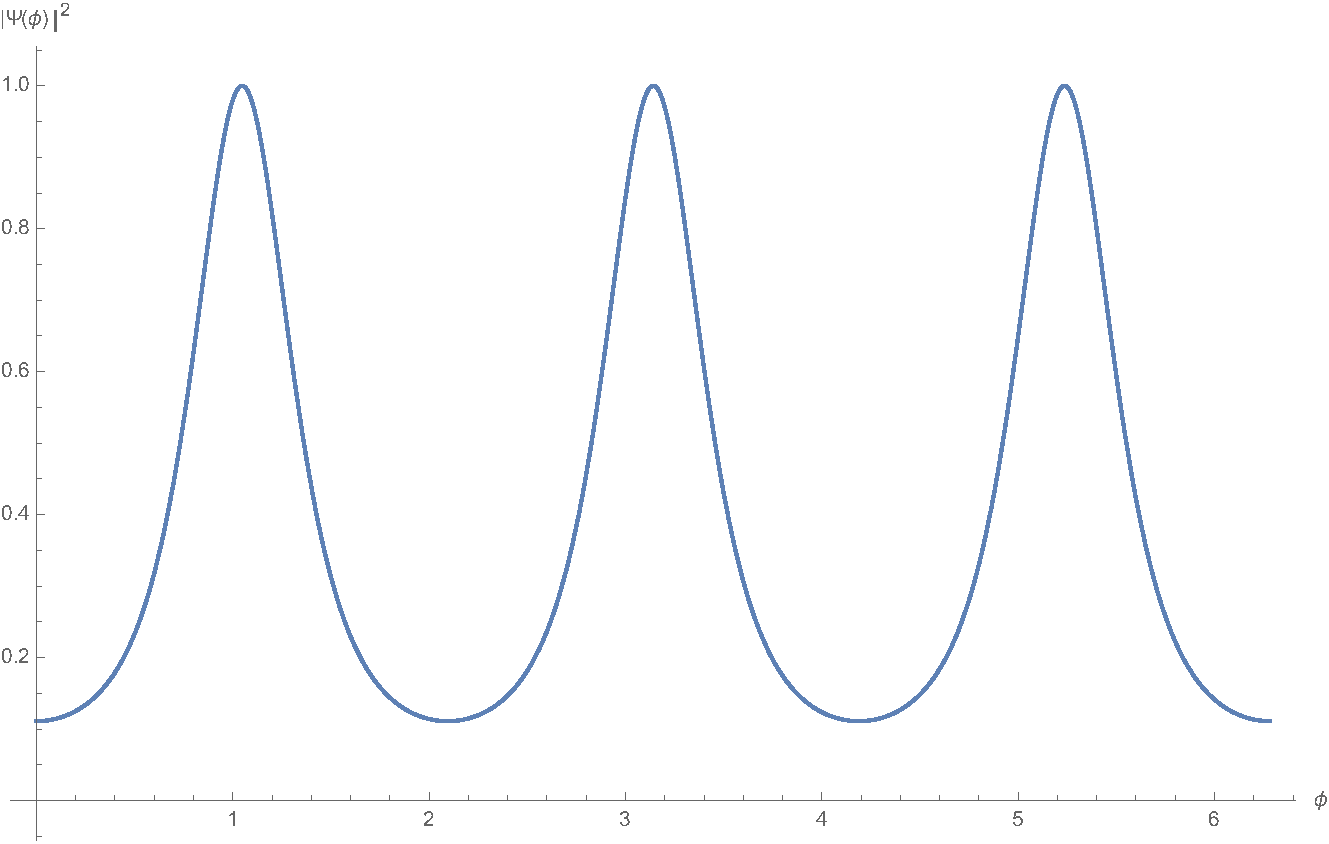
\includegraphics[width=0.75\columnwidth]{prob_density_graph.pdf}
      \end{figure}

      \noindent The fact that this plot is periodic at $0$ and $2\pi$ should convince you
      that $|\Psi\rangle$ is a valid state for a particle on the ring.\\

      
    \item Determine the normalization constant N. \\
      
      \noindent We can not easily rewrite the wave function $\Psi(\phi)$ in terms
      of the eigenstates $\Phi_m(\phi)$. The best approach is to stay in
      function land and use the integral representation of the inner product.
      That is,

      \begin{align}
        1 &= \langle \Psi | \Psi \rangle = \int\limits_0^{2\pi}\left| \frac{N}{[2+3\cos\phi]^2} \right|^2r_0d\phi \\
          &= |N|^2r_0\int\limits_0^{2\pi}\frac{1}{4+4\cos3\phi+\cos^23\phi}d\phi \\
        &= |N|^2r_0\left[ \frac{4}{9\sqrt{3}}\tan^{-1}\left( \frac{1}{\sqrt{3}}\tan\frac{3\phi}{2} \right)-\frac{\sin3\phi}{9(2+\cos(3\phi))} \right]_0^{2\pi}
      \end{align}
      Directly plugging in $2\pi$ and $0$ in order to evaluate (3) yields a
      value of 0. That is \textbf{wrong}. In part (a) we graphed the integrand.
      It is a perfectly well behaved function; it's smooth and doesn't blow up.
      In fact, the problem is that the
      antiderivative involves a term of the form $\tan^{-1}(\tan(x))$. This is
      \textbf{not} well defined over the entire interval $[0, 2\pi]$ because the
      inverse tangent function has a restricted range from $(-\pi/2, \pi/2)$. If
      you are not convinced, try graphing $\tan^{-1}(\tan(x))$ and the
      indefinite integral from equation (3).  \\

      To get around this problem, we can recognize that there is symmetry in our graph from
      part (a).  Instead, let's integrate from $0$ to $2\pi/6$ and then multiply by 6.
      \begin{align}
        1 &= 6|N|^2r_0 \left[ \frac{4}{9\sqrt{3}}\tan^{-1}\left( \frac{1}{\sqrt{3}}\tan\frac{3\phi}{2} \right)-\frac{\sin3\phi}{9(2+\cos(3\phi))} \right]_0^{2\pi/6} \\
          &= 6|N|^2r_0\left[ \frac{4}{9\sqrt{3}} \frac{\pi}{2}\right] = |N|^2r_0\left[ \frac{4\pi}{3\sqrt{3}} \right] \\
        \Rightarrow N &= \sqrt{\frac{3\sqrt{3}}{4\pi r_0}}
      \end{align}
      The normalized wave function is therefore
      \begin{equation}
        \Psi(\phi) = \sqrt{\frac{3\sqrt{3}}{4\pi r_0}}\;\frac{1}{2+\cos3\phi}
      \end{equation}
      \vspace{2em}
      
    \item  Plot the wave function\\
      \noindent A plot of our result from (b) is shown below. Note that we have
      set $r_0 = 1$ for convenience. 
      
       \begin{figure}[!hbt]
        \centering
        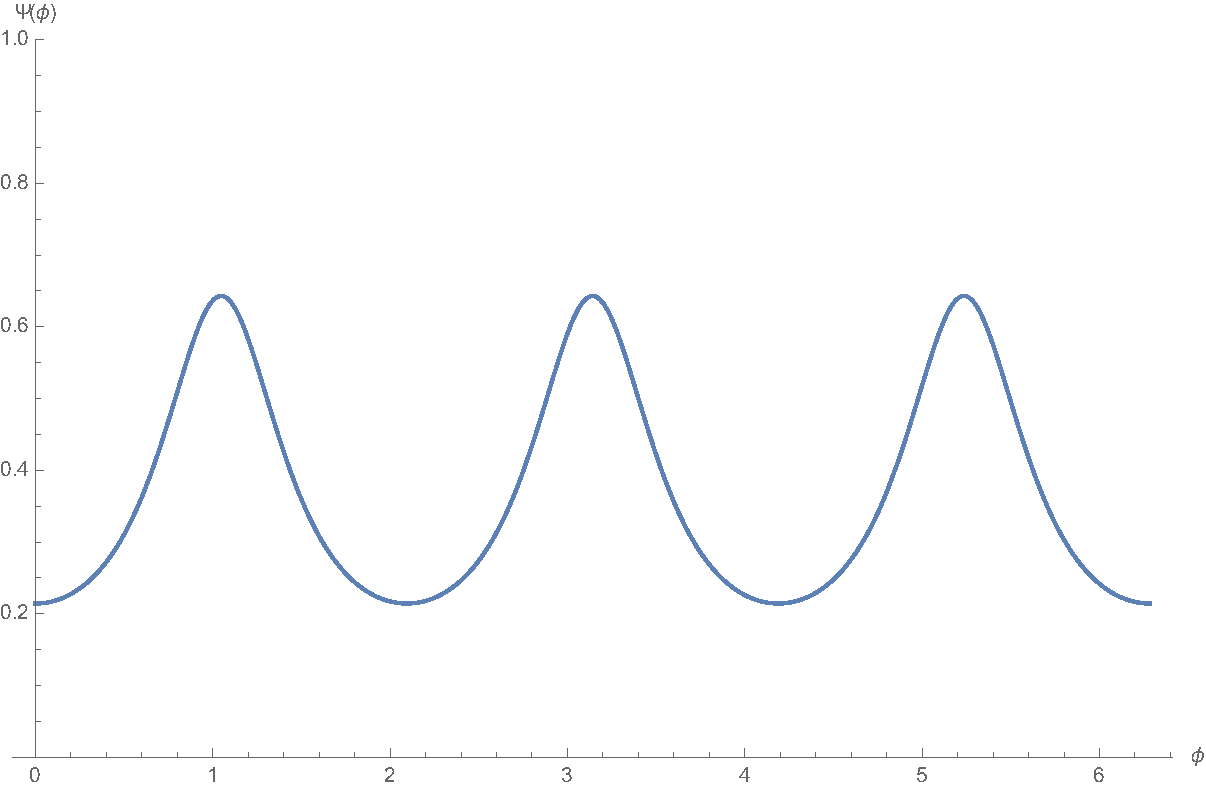
\includegraphics[width=0.9\columnwidth]{wavefunction_graph.pdf}
      \end{figure}

    \item What is the expectation value of $L_z$ in this state? \\
      \noindent The expecation value is
      \begin{align}
        \left\langle L_z \right\rangle &= \left\langle \Psi | L_z | \Psi \right\rangle   \\
                                       &= \int\limits_0^{2\pi} \Psi^*(\phi)\left( -i\hbar\frac{\partial}{\partial \phi} \right)\Psi(\phi)r_0 d\phi \\
                                       &= \frac{3\sqrt{3}}{4\pi r_0}\int\limits_0^{2\pi}\frac{1}{2+\cos3\phi}\left( -i\hbar\frac{\partial}{\partial \phi} \right)\frac{1}{2+\cos3\phi}r_0d\phi \\
                                       &= -i\hbar\frac{3\sqrt{3}}{4\pi}\int\limits_0^{2\pi}\frac{3\sin3\phi}{2+\cos3\phi}d\phi  \\
        &= 0
      \end{align}
    \end{enumerate}
\end{enumerate}
\end{document}

